\documentclass[11pt,a4paper]{article}
\usepackage[brazil]{babel}
\usepackage[utf8]{inputenc}
\usepackage{amsmath,amssymb,amsfonts}
\usepackage{graphicx}
\usepackage{booktabs}
\usepackage{geometry}
\usepackage{hyperref}
\usepackage{subcaption}
\usepackage{cite}

\geometry{top=2.5cm, bottom=2.5cm, left=2.5cm, right=2.5cm}

\title{\textbf{Trabalho Prático 1: Regressão Simbólica com Programação Genética}}
\author{[Nome do Aluno -- Matrícula]\\
\textit{Departamento de Ciência da Computação}\\
\textit{Universidade Federal de Minas Gerais (UFMG)}}
\date{\today}

\begin{document}
\maketitle

\begin{abstract}
% [ORIENTAÇÃO: Resumo conciso de até 200 palavras descrevendo o objetivo do trabalho,
% os métodos de programação genética implementados, os experimentos realizados sobre as bases
% synth1, synth2 e concrete com 30 repetições, e as principais conclusões obtidas.]
\end{abstract}

\section{Introdução}
% [ORIENTAÇÃO: Contextualize o problema de regressão simbólica e diferencie-o da regressão clássica.
% Apresente a motivação para o uso de Programação Genética (PG).
% Declare os objetivos do trabalho: investigar o impacto de hiperparâmetros (tamanho da população e gerações),
% métodos de seleção (Torneio, Roleta Escalonada, epsilon-Lexicase), operadores de variação (crossover vs. mutação)
% e elitismo, finalizando com a validação em bases sintéticas e reais.
% Descreva a organização das seções seguintes do relatório.]

\section{Implementação}
% [ORIENTAÇÃO: Detalhe as decisões de engenharia e modelagem matemática do framework de PG.]

\subsection{Representação dos Indivíduos e Inicialização}
% [ORIENTAÇÃO: Descreva a árvore sintática baseada em nós, a restrição rígida de profundidade máxima igual a 7,
% e a inicialização Ramped Half-and-Half (profundidades de 2 a 5 com método grow e full).]

\subsection{Conjunto Primitivo e Terminais}
% [ORIENTAÇÃO: Apresente as funções primitivas (+, -, *, divisão protegida, sin, cos, log protegido, exp protegido)
% e justifique as proteções numéricas contra divisões por zero e overflow.
% Descreva as variáveis terminais (X0 a XD-1) e as constantes efêmeras (ERCs) com perturbação gaussiana.]

\subsection{Função de Fitness e Avaliação Vetorizada}
% [ORIENTAÇÃO: Apresente a fórmula da Raiz do Erro Quadrático Médio (RMSE).
% Explique como a avaliação foi vetorizada com NumPy sobre matrizes N x D.]

\subsection{Operadores de Seleção}
% [ORIENTAÇÃO: Descreva formalmente os três operadores de seleção:
% 1. Torneio com k=2.
% 2. Roleta com escalonamento linear (f_max - f_i + delta) para minimização.
% 3. epsilon-Lexicase com limiar dinâmico baseado no Desvio Absoluto Mediano (MAD) por caso de teste.]

\subsection{Operadores de Variação e Esquema Reprodutivo}
% [ORIENTAÇÃO: Explique a seleção mutuamente exclusiva de operadores por vaga na nova população (pc, pm, cloning).
% Detalhe o crossover de subárvore com rejeição por profundidade > 7 e a mutação por perturbação ou subárvore.
% Explique o mecanismo de elitismo preservando o melhor indivíduo.]

\section{Experimentos e Análise de Resultados}
% [ORIENTAÇÃO: Detalhe o protocolo experimental: 30 sementes aleatórias por configuração,
% divisões de treino e teste, e métricas coletadas.]

\subsection{Impacto do Tamanho da População e Número de Gerações (Passo 1)}
% [ORIENTAÇÃO: Analise o compromisso entre tamanho da população, número de gerações e custo computacional.
% Discuta se configurações com mais gerações apresentaram overfitting ou bloat.]

% Inserção da Tabela 1:
% \begin{table}[htbp]
  \centering
  \caption{Resultados resumidos do Passo 1}
  \label{tab:step1}
  \begin{tabular}{llcccc}
    \toprule
    Configuration & Dataset & Train RMSE & Test RMSE & Avg Nodes & Avg Depth \\
    \midrule
    pop100\_gen100 & synth1 & 3.7115 $\pm$ 1.6265 & 5.1047 $\pm$ 2.9038 & 27.83 $\pm$ 7.36 & 6.80 $\pm$ 0.48 \\
    pop100\_gen50 & synth1 & 5.8387 $\pm$ 2.5500 & 8.1907 $\pm$ 4.4497 & 22.70 $\pm$ 7.51 & 6.63 $\pm$ 0.81 \\
    pop100\_gen500 & synth1 & 2.1603 $\pm$ 1.0587 & 3.4942 $\pm$ 2.2174 & 37.70 $\pm$ 10.63 & 7.00 $\pm$ 0.00 \\
    pop500\_gen100 & synth1 & 2.6846 $\pm$ 1.0071 & 3.6628 $\pm$ 1.5426 & 30.80 $\pm$ 10.39 & 6.93 $\pm$ 0.25 \\
    pop500\_gen50 & synth1 & 4.0013 $\pm$ 1.4413 & 5.3800 $\pm$ 2.4275 & 22.20 $\pm$ 7.51 & 6.73 $\pm$ 0.52 \\
    pop500\_gen500 & synth1 & 1.4166 $\pm$ 0.6404 & 2.4171 $\pm$ 2.2293 & 40.33 $\pm$ 10.92 & 6.97 $\pm$ 0.18 \\
    pop50\_gen100 & synth1 & 6.7725 $\pm$ 4.1735 & 15.4066 $\pm$ 31.8452 & 26.90 $\pm$ 12.08 & 6.63 $\pm$ 1.07 \\
    pop50\_gen50 & synth1 & 10.0751 $\pm$ 5.1096 & 14.4915 $\pm$ 7.9374 & 20.33 $\pm$ 9.66 & 6.30 $\pm$ 1.15 \\
    pop50\_gen500 & synth1 & 3.2806 $\pm$ 2.0302 & 4.9290 $\pm$ 3.1681 & 36.97 $\pm$ 10.23 & 6.97 $\pm$ 0.18 \\
    \bottomrule
  \end{tabular}
\end{table}


% Inserção da Figura 1 (Convergência e Bloat no Passo 1):
\begin{figure}[htbp]
  \centering
  \IfFileExists{results/plots/fig1_step1_convergence.png}{%
    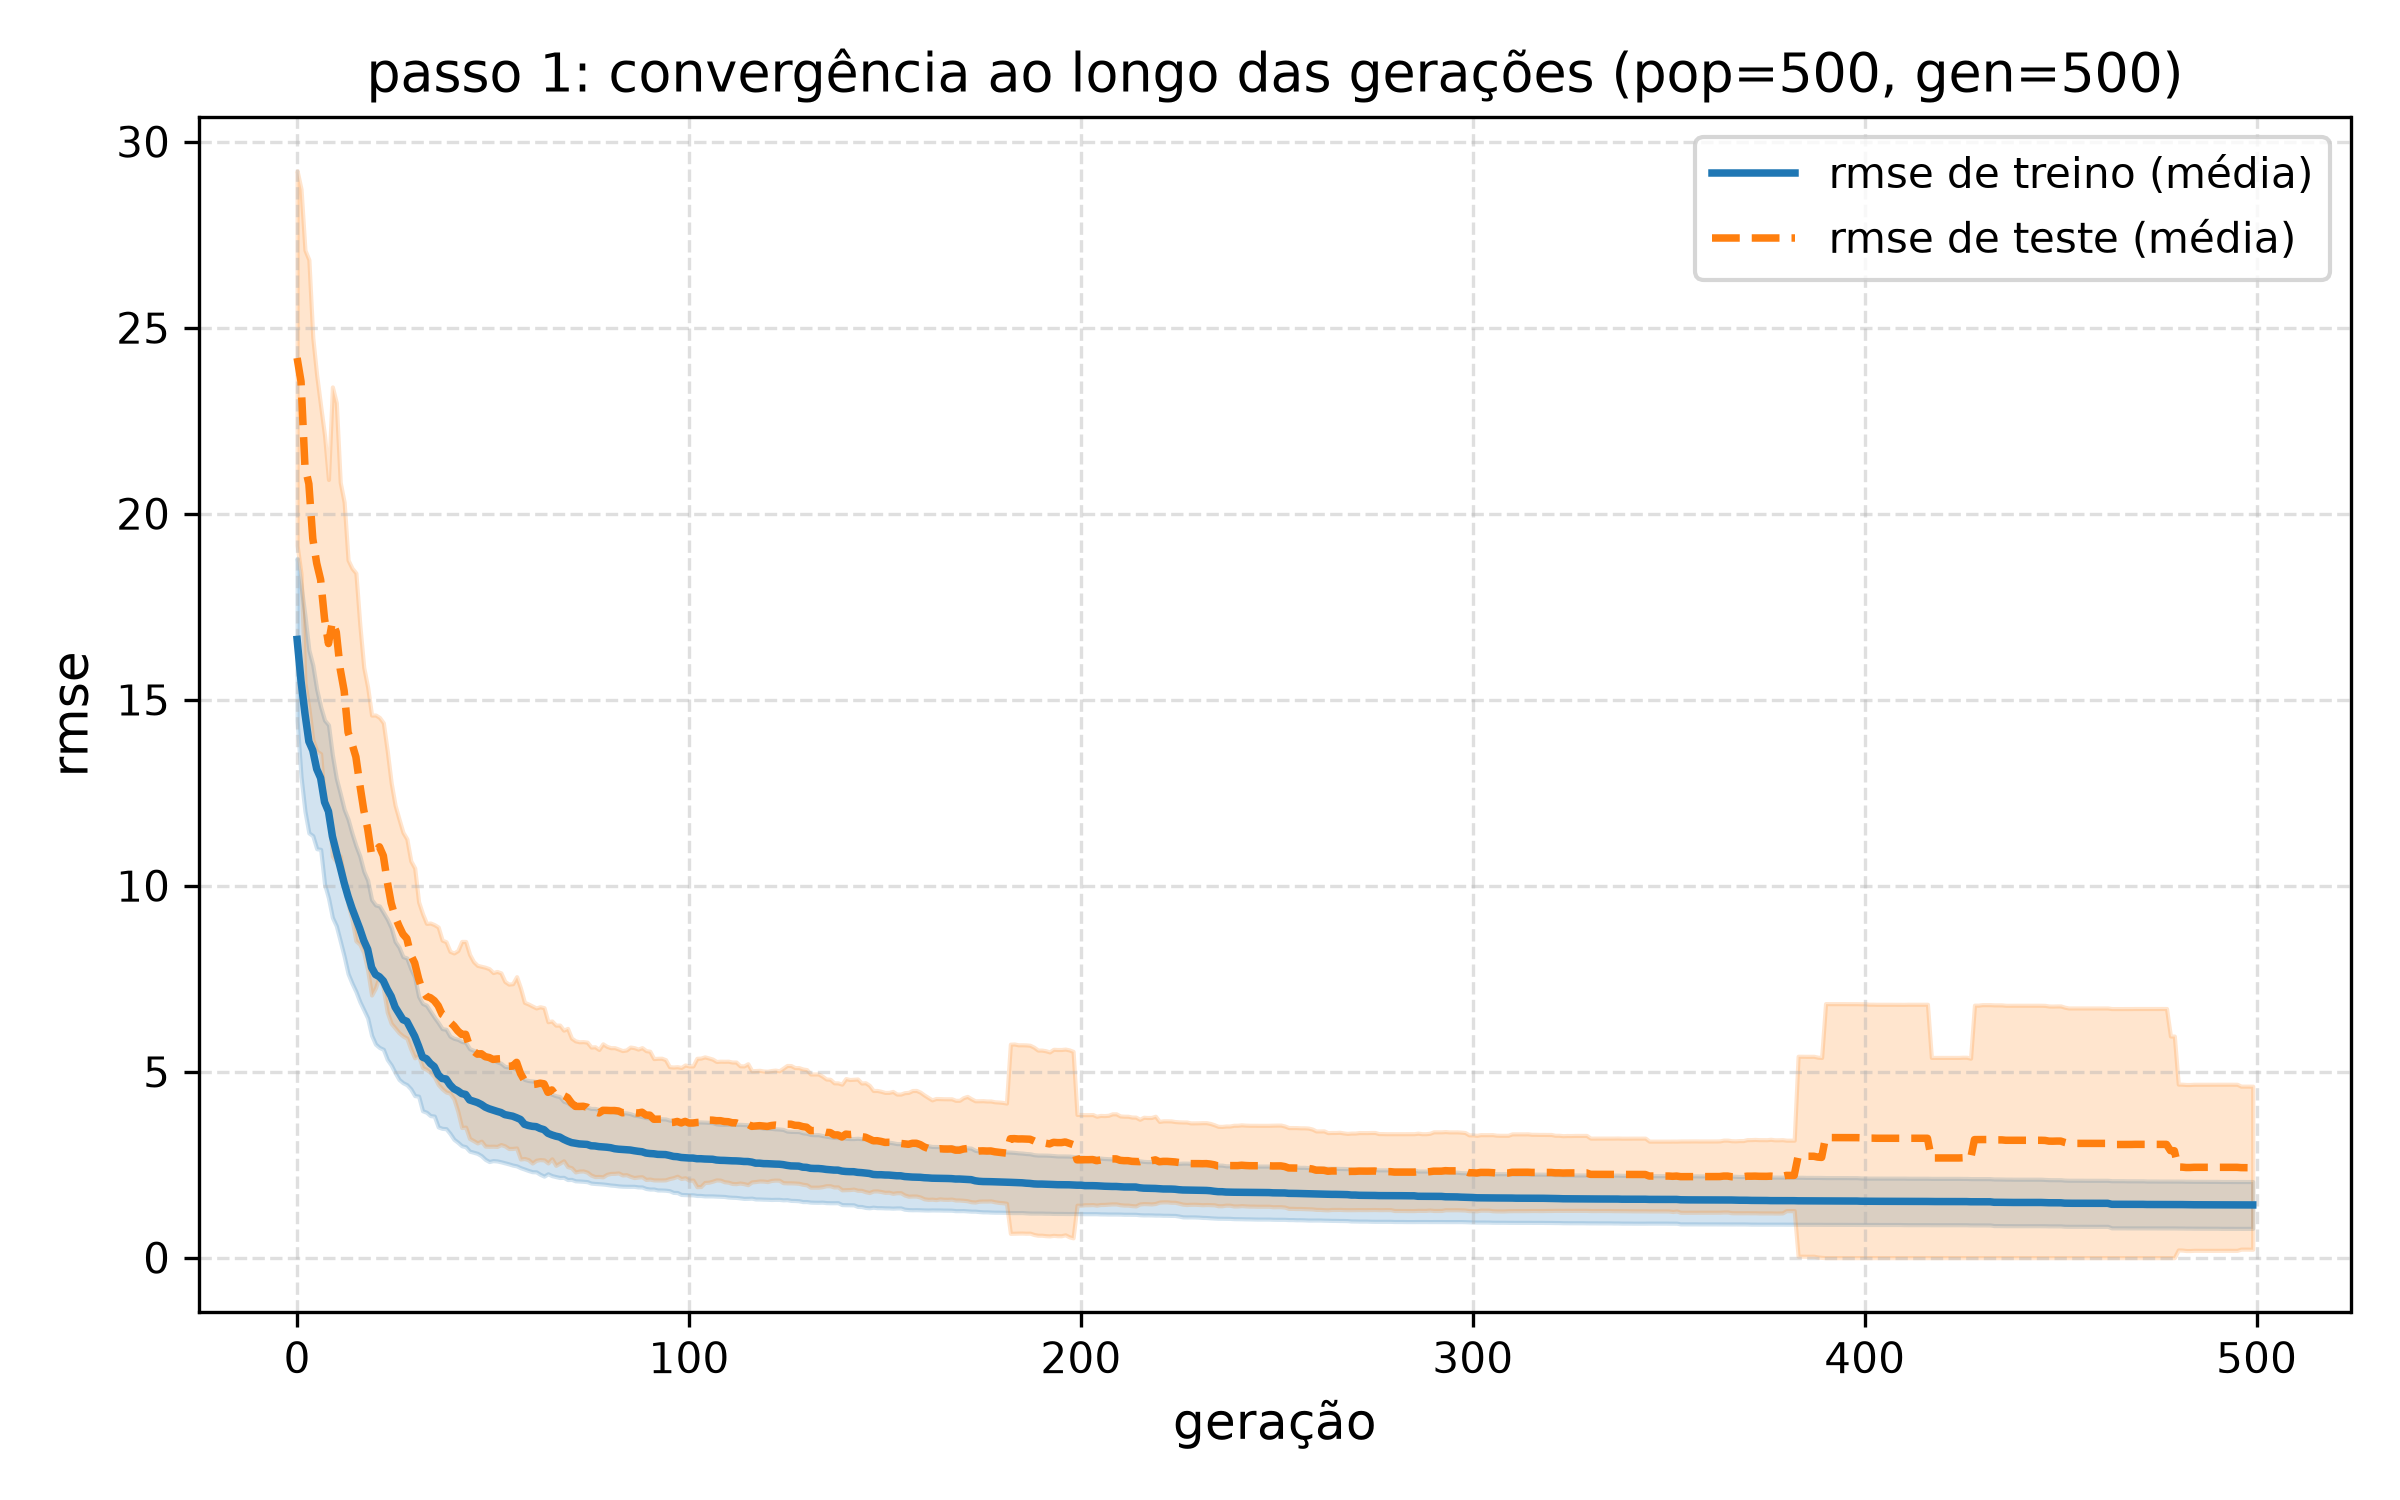
\includegraphics[width=0.85\textwidth]{results/plots/fig1_step1_convergence.png}%
  }{%
    \fbox{\parbox{0.8\textwidth}{\centering Placeholder: Inserir \texttt{results/plots/fig1_step1_convergence.png}}}%
  }
  \caption{Convergência do RMSE de treino e teste ao longo das gerações para diferentes tamanhos de população e gerações.}
  \label{fig:step1_convergence}
\end{figure}

\begin{figure}[htbp]
  \centering
  \IfFileExists{results/plots/fig2_step1_bloat.png}{%
    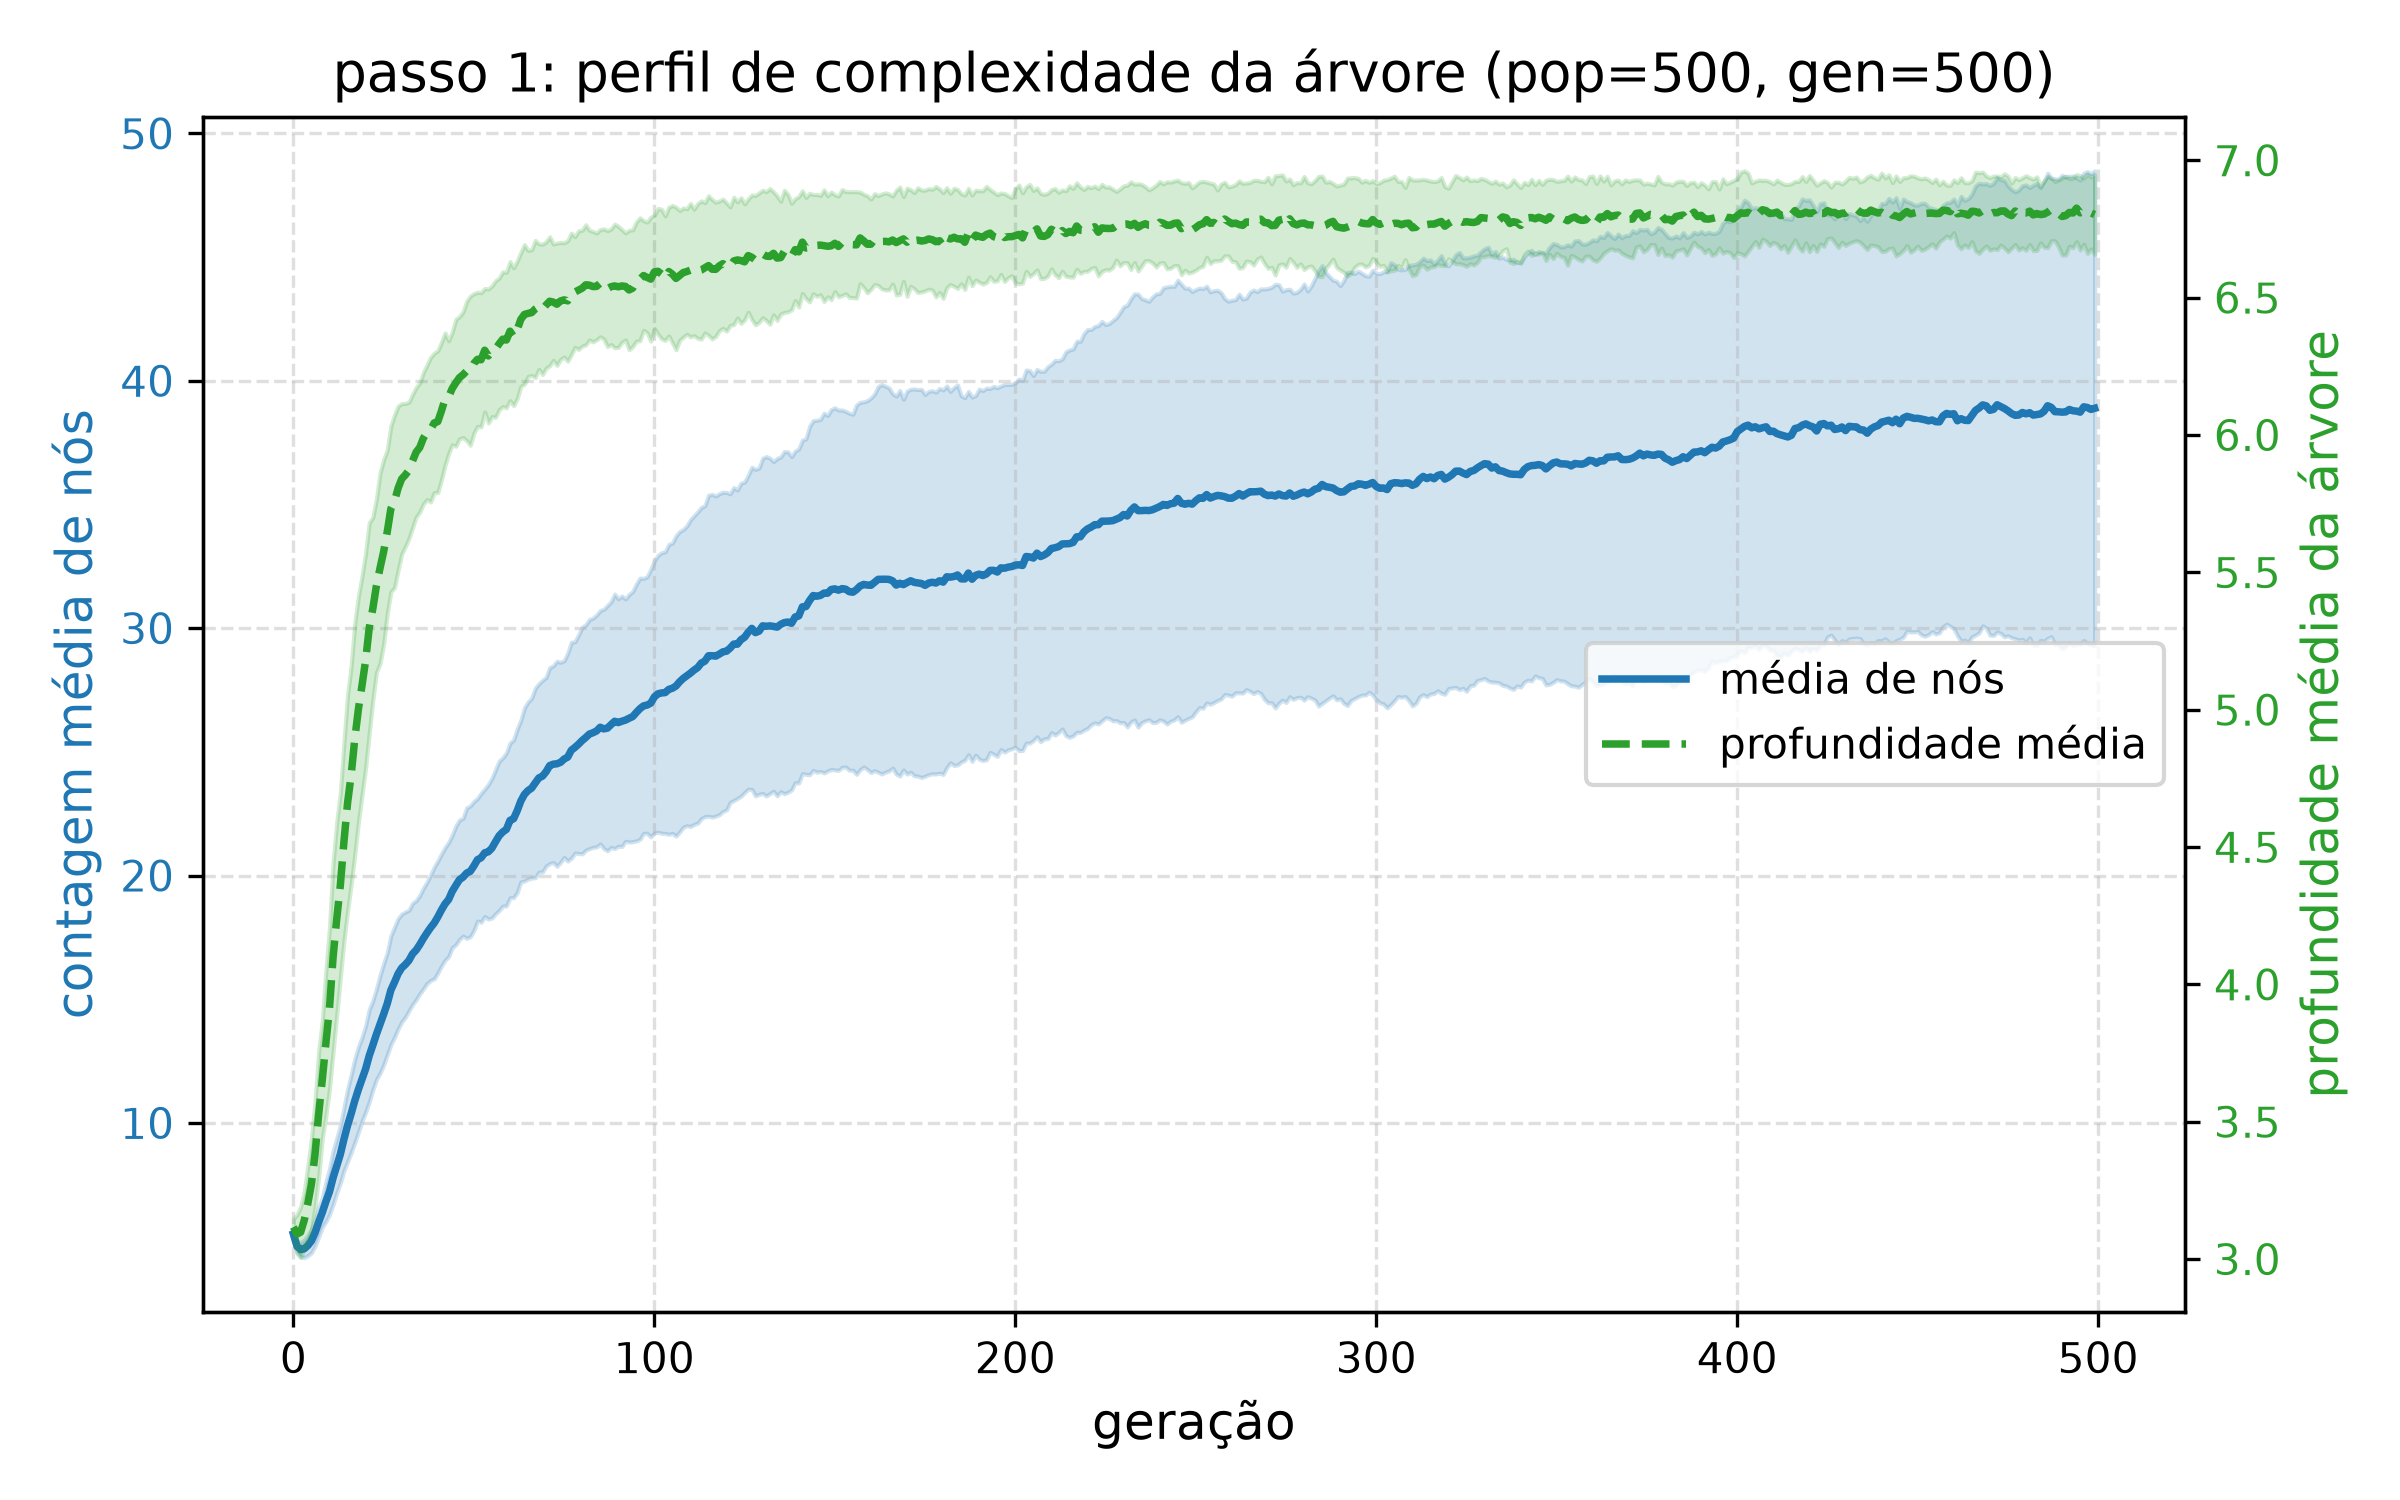
\includegraphics[width=0.85\textwidth]{results/plots/fig2_step1_bloat.png}%
  }{%
    \fbox{\parbox{0.8\textwidth}{\centering Placeholder: Inserir \texttt{results/plots/fig2_step1_bloat.png}}}%
  }
  \caption{Evolução do número médio de nós e profundidade média (análise de bloat) no Passo 1.}
  \label{fig:step1_bloat}
\end{figure}

\subsection{Comparação dos Métodos de Seleção (Passo 2)}
% [ORIENTAÇÃO: Compare Torneio (k=2), Roleta Escalonada e epsilon-Lexicase.
% Discuta a pressão seletiva, a preservação da diversidade estrutural (árvores canônicas únicas)
% e a capacidade de escapar de mínimos locais.]

% Inserção da Tabela 2:
% \begin{table}[htbp]
  \centering
  \caption{Resultados resumidos do Passo 2}
  \label{tab:step2}
  \begin{tabular}{llcccc}
    \toprule
    Configuration & Dataset & Train RMSE & Test RMSE & Avg Nodes & Avg Depth \\
    \midrule
    lexicase & synth1 & 0.2609 $\pm$ 0.3722 & 0.4927 $\pm$ 0.9241 & 36.27 $\pm$ 9.10 & 7.00 $\pm$ 0.00 \\
    roulette & synth1 & 4.0158 $\pm$ 2.1606 & 6.1381 $\pm$ 4.1907 & 13.43 $\pm$ 4.26 & 6.00 $\pm$ 0.95 \\
    tournament & synth1 & 1.4166 $\pm$ 0.6404 & 2.4171 $\pm$ 2.2293 & 40.33 $\pm$ 10.92 & 6.97 $\pm$ 0.18 \\
    \bottomrule
  \end{tabular}
\end{table}


% Inserção da Figura 2 (Convergência e Diversidade na Seleção):
\begin{figure}[htbp]
  \centering
  \IfFileExists{results/plots/fig3_step2_selection_convergence.png}{%
    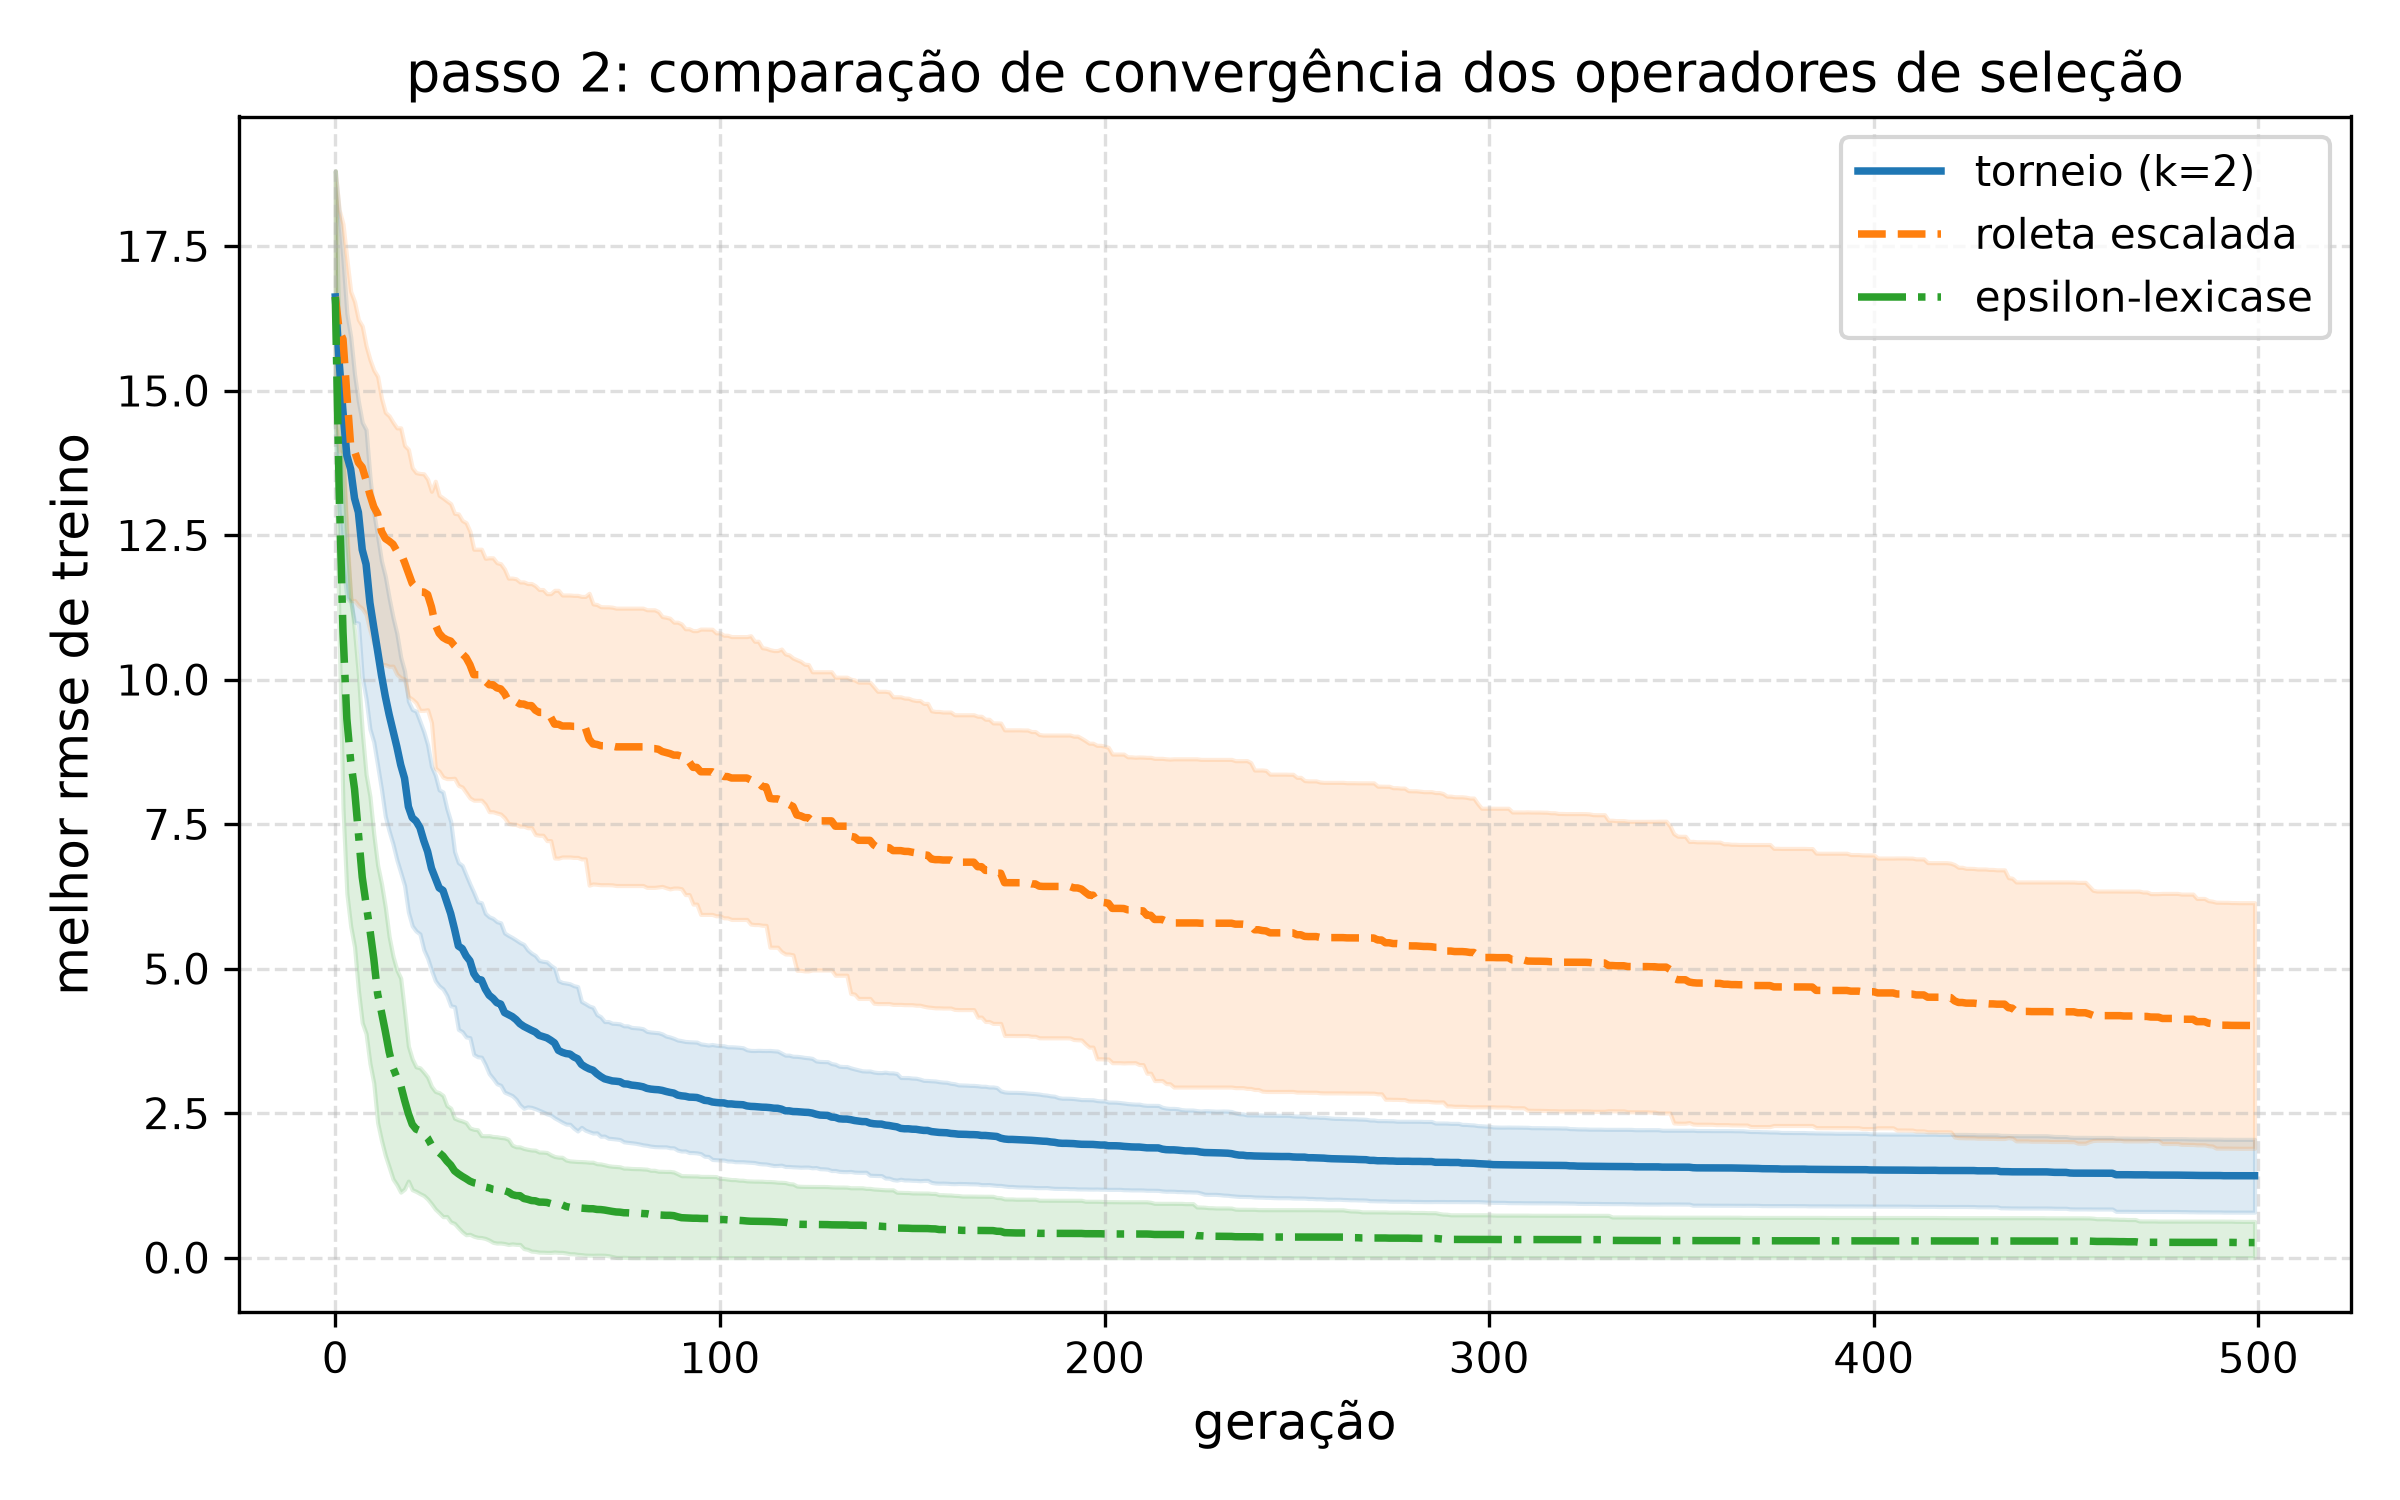
\includegraphics[width=0.85\textwidth]{results/plots/fig3_step2_selection_convergence.png}%
  }{%
    \fbox{\parbox{0.8\textwidth}{\centering Placeholder: Inserir \texttt{results/plots/fig3_step2_selection_convergence.png}}}%
  }
  \caption{Comparação da convergência do melhor RMSE de treino entre Torneio, Roleta Escalonada e $\epsilon$-Lexicase.}
  \label{fig:step2_selection}
\end{figure}

\begin{figure}[htbp]
  \centering
  \IfFileExists{results/plots/fig4_step2_diversity.png}{%
    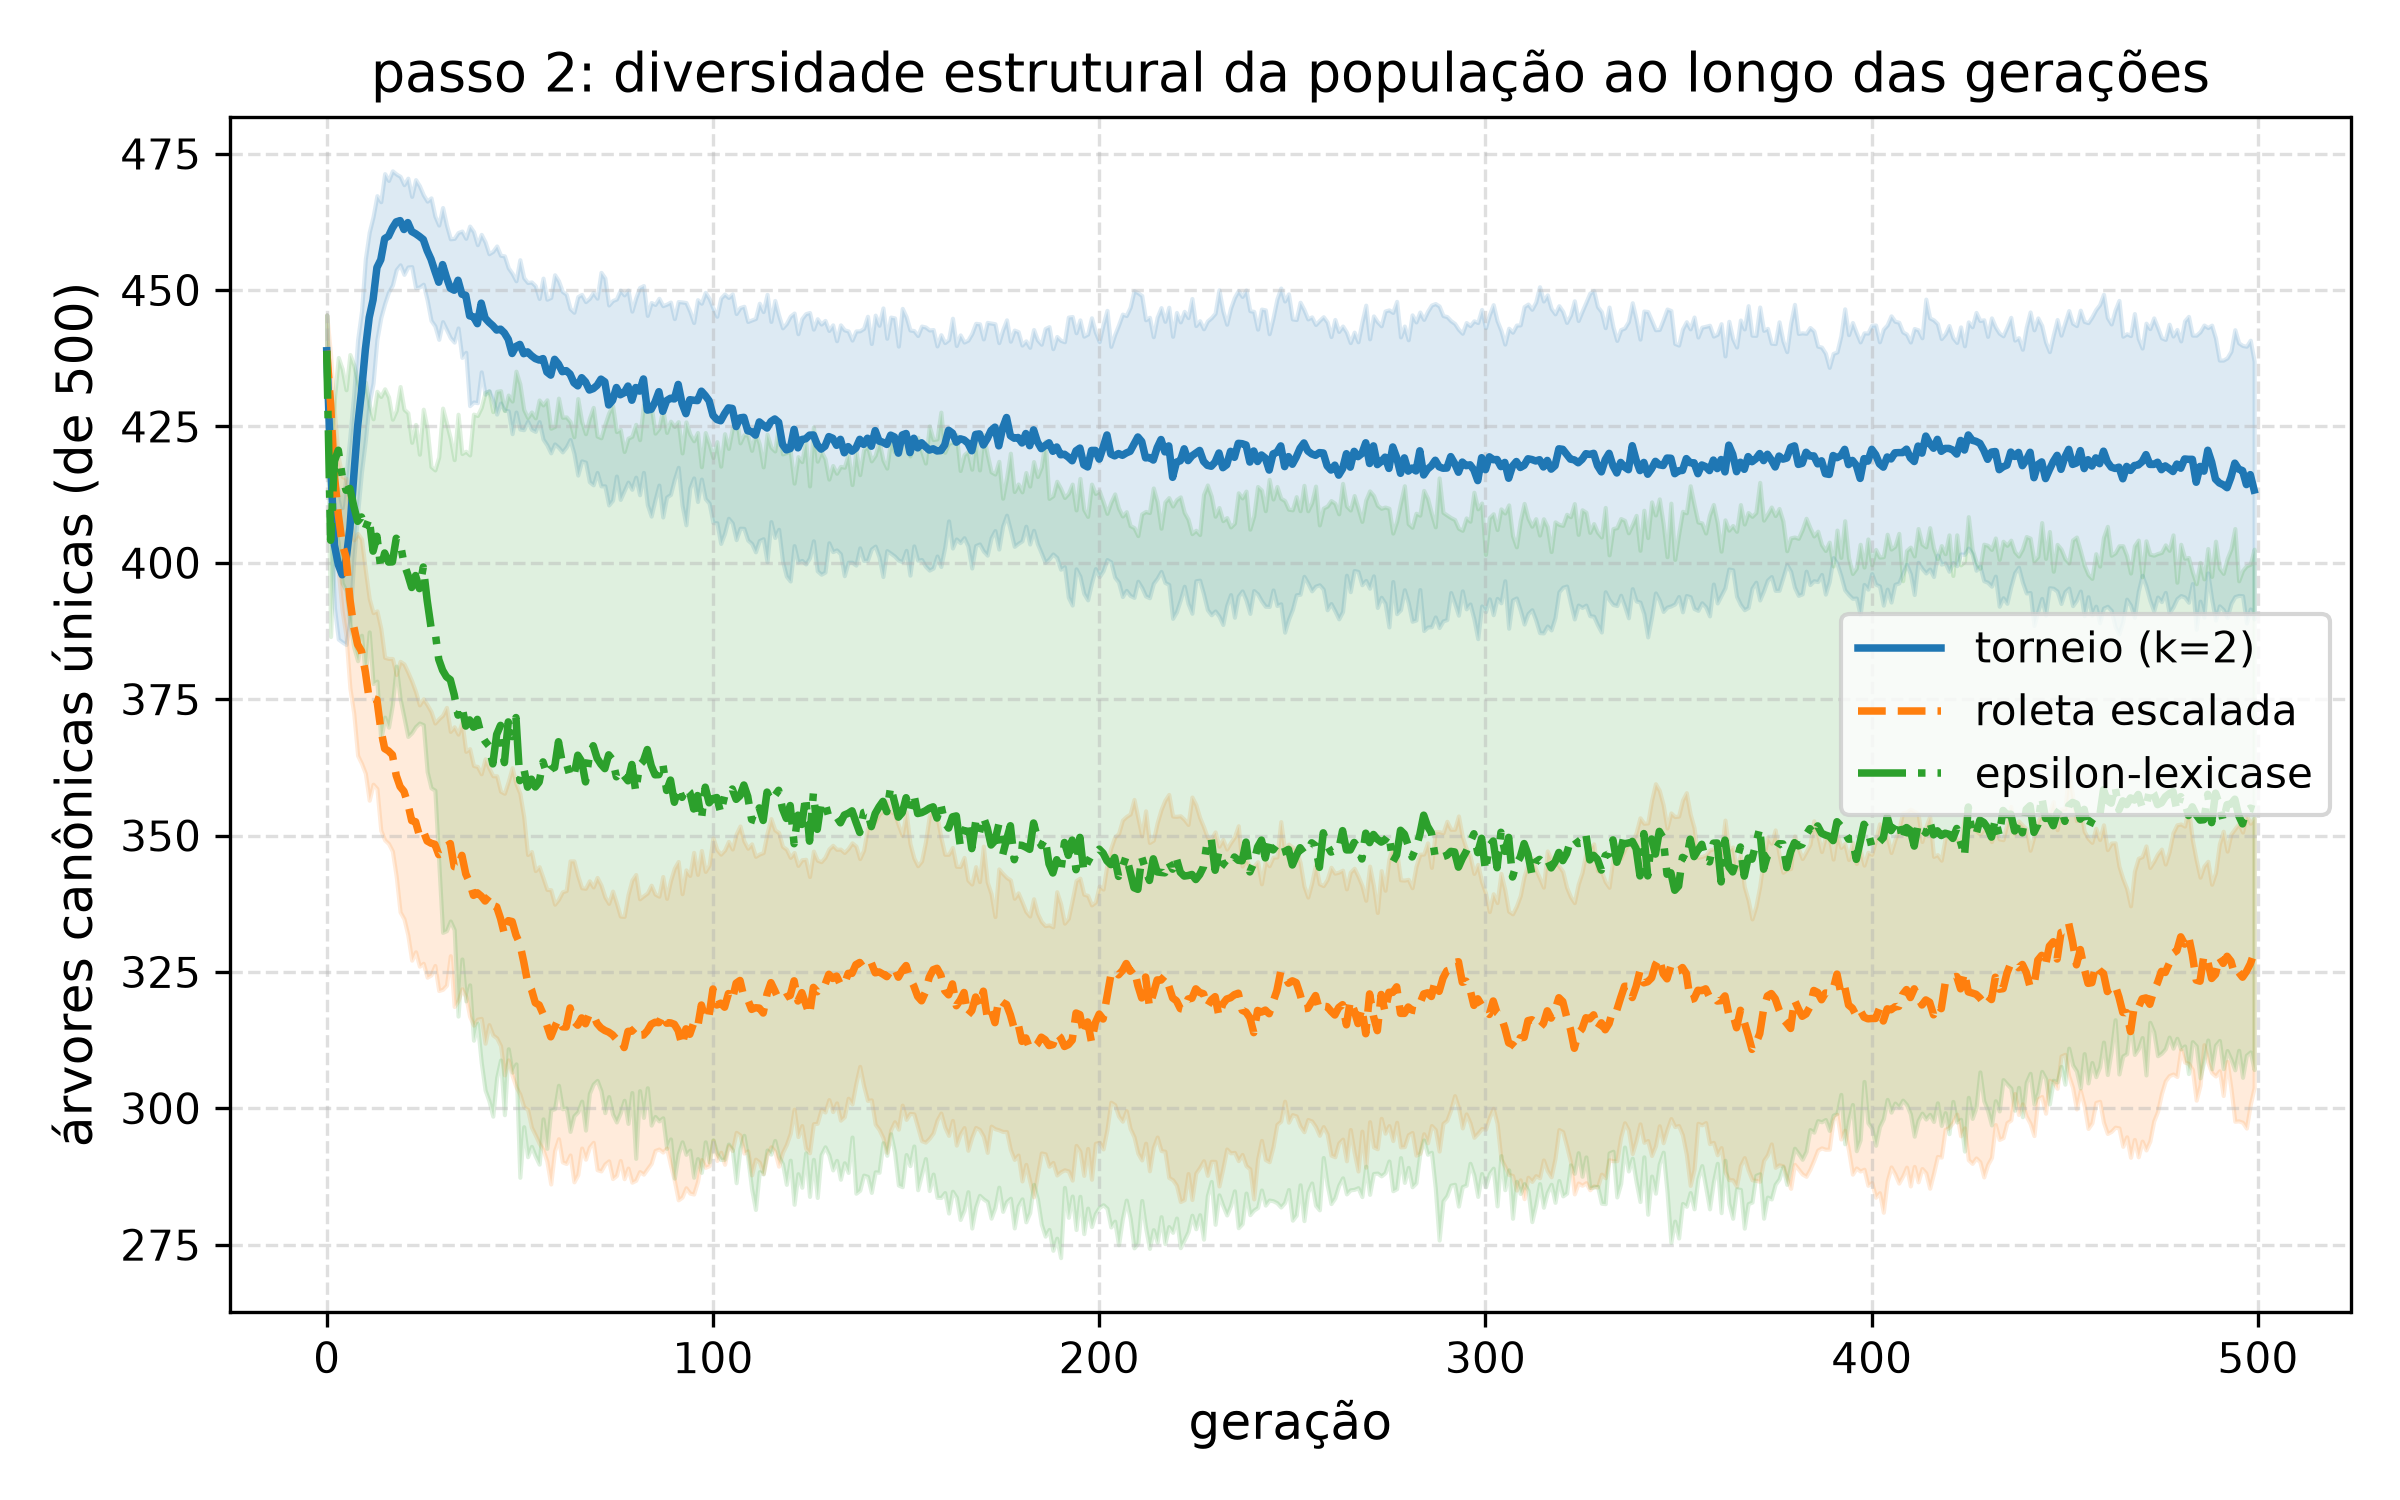
\includegraphics[width=0.85\textwidth]{results/plots/fig4_step2_diversity.png}%
  }{%
    \fbox{\parbox{0.8\textwidth}{\centering Placeholder: Inserir \texttt{results/plots/fig4_step2_diversity.png}}}%
  }
  \caption{Evolução da diversidade populacional (contagem de indivíduos sintaticamente únicos).}
  \label{fig:step2_diversity}
\end{figure}

\subsection{Comparação dos Operadores de Variação (Passo 3)}
% [ORIENTAÇÃO: Compare a configuração de alto crossover (pc=0.9, pm=0.05) com a de alta mutação (pc=0.6, pm=0.30).
% Analise a taxa de sucesso do crossover (filhos melhores vs. piores que a média dos pais) e seu impacto no bloat.]

% Inserção da Tabela 3:
% \begin{table}[htbp]
  \centering
  \caption{Resultados resumidos do Passo 3}
  \label{tab:step3}
  \begin{tabular}{llcccc}
    \toprule
    Configuration & Dataset & Train RMSE & Test RMSE & Avg Nodes & Avg Depth \\
    \midrule
    pc60\_pm30 & synth1 & 0.4487 $\pm$ 0.4988 & 0.8934 $\pm$ 1.3282 & 32.40 $\pm$ 5.97 & 6.93 $\pm$ 0.25 \\
    pc90\_pm05 & synth1 & 0.2609 $\pm$ 0.3722 & 0.4927 $\pm$ 0.9241 & 36.27 $\pm$ 9.10 & 7.00 $\pm$ 0.00 \\
    \bottomrule
  \end{tabular}
\end{table}


% Inserção da Figura 3 (Sucesso do Crossover):
\begin{figure}[htbp]
  \centering
  \IfFileExists{results/plots/fig5_step3_operator_success.png}{%
    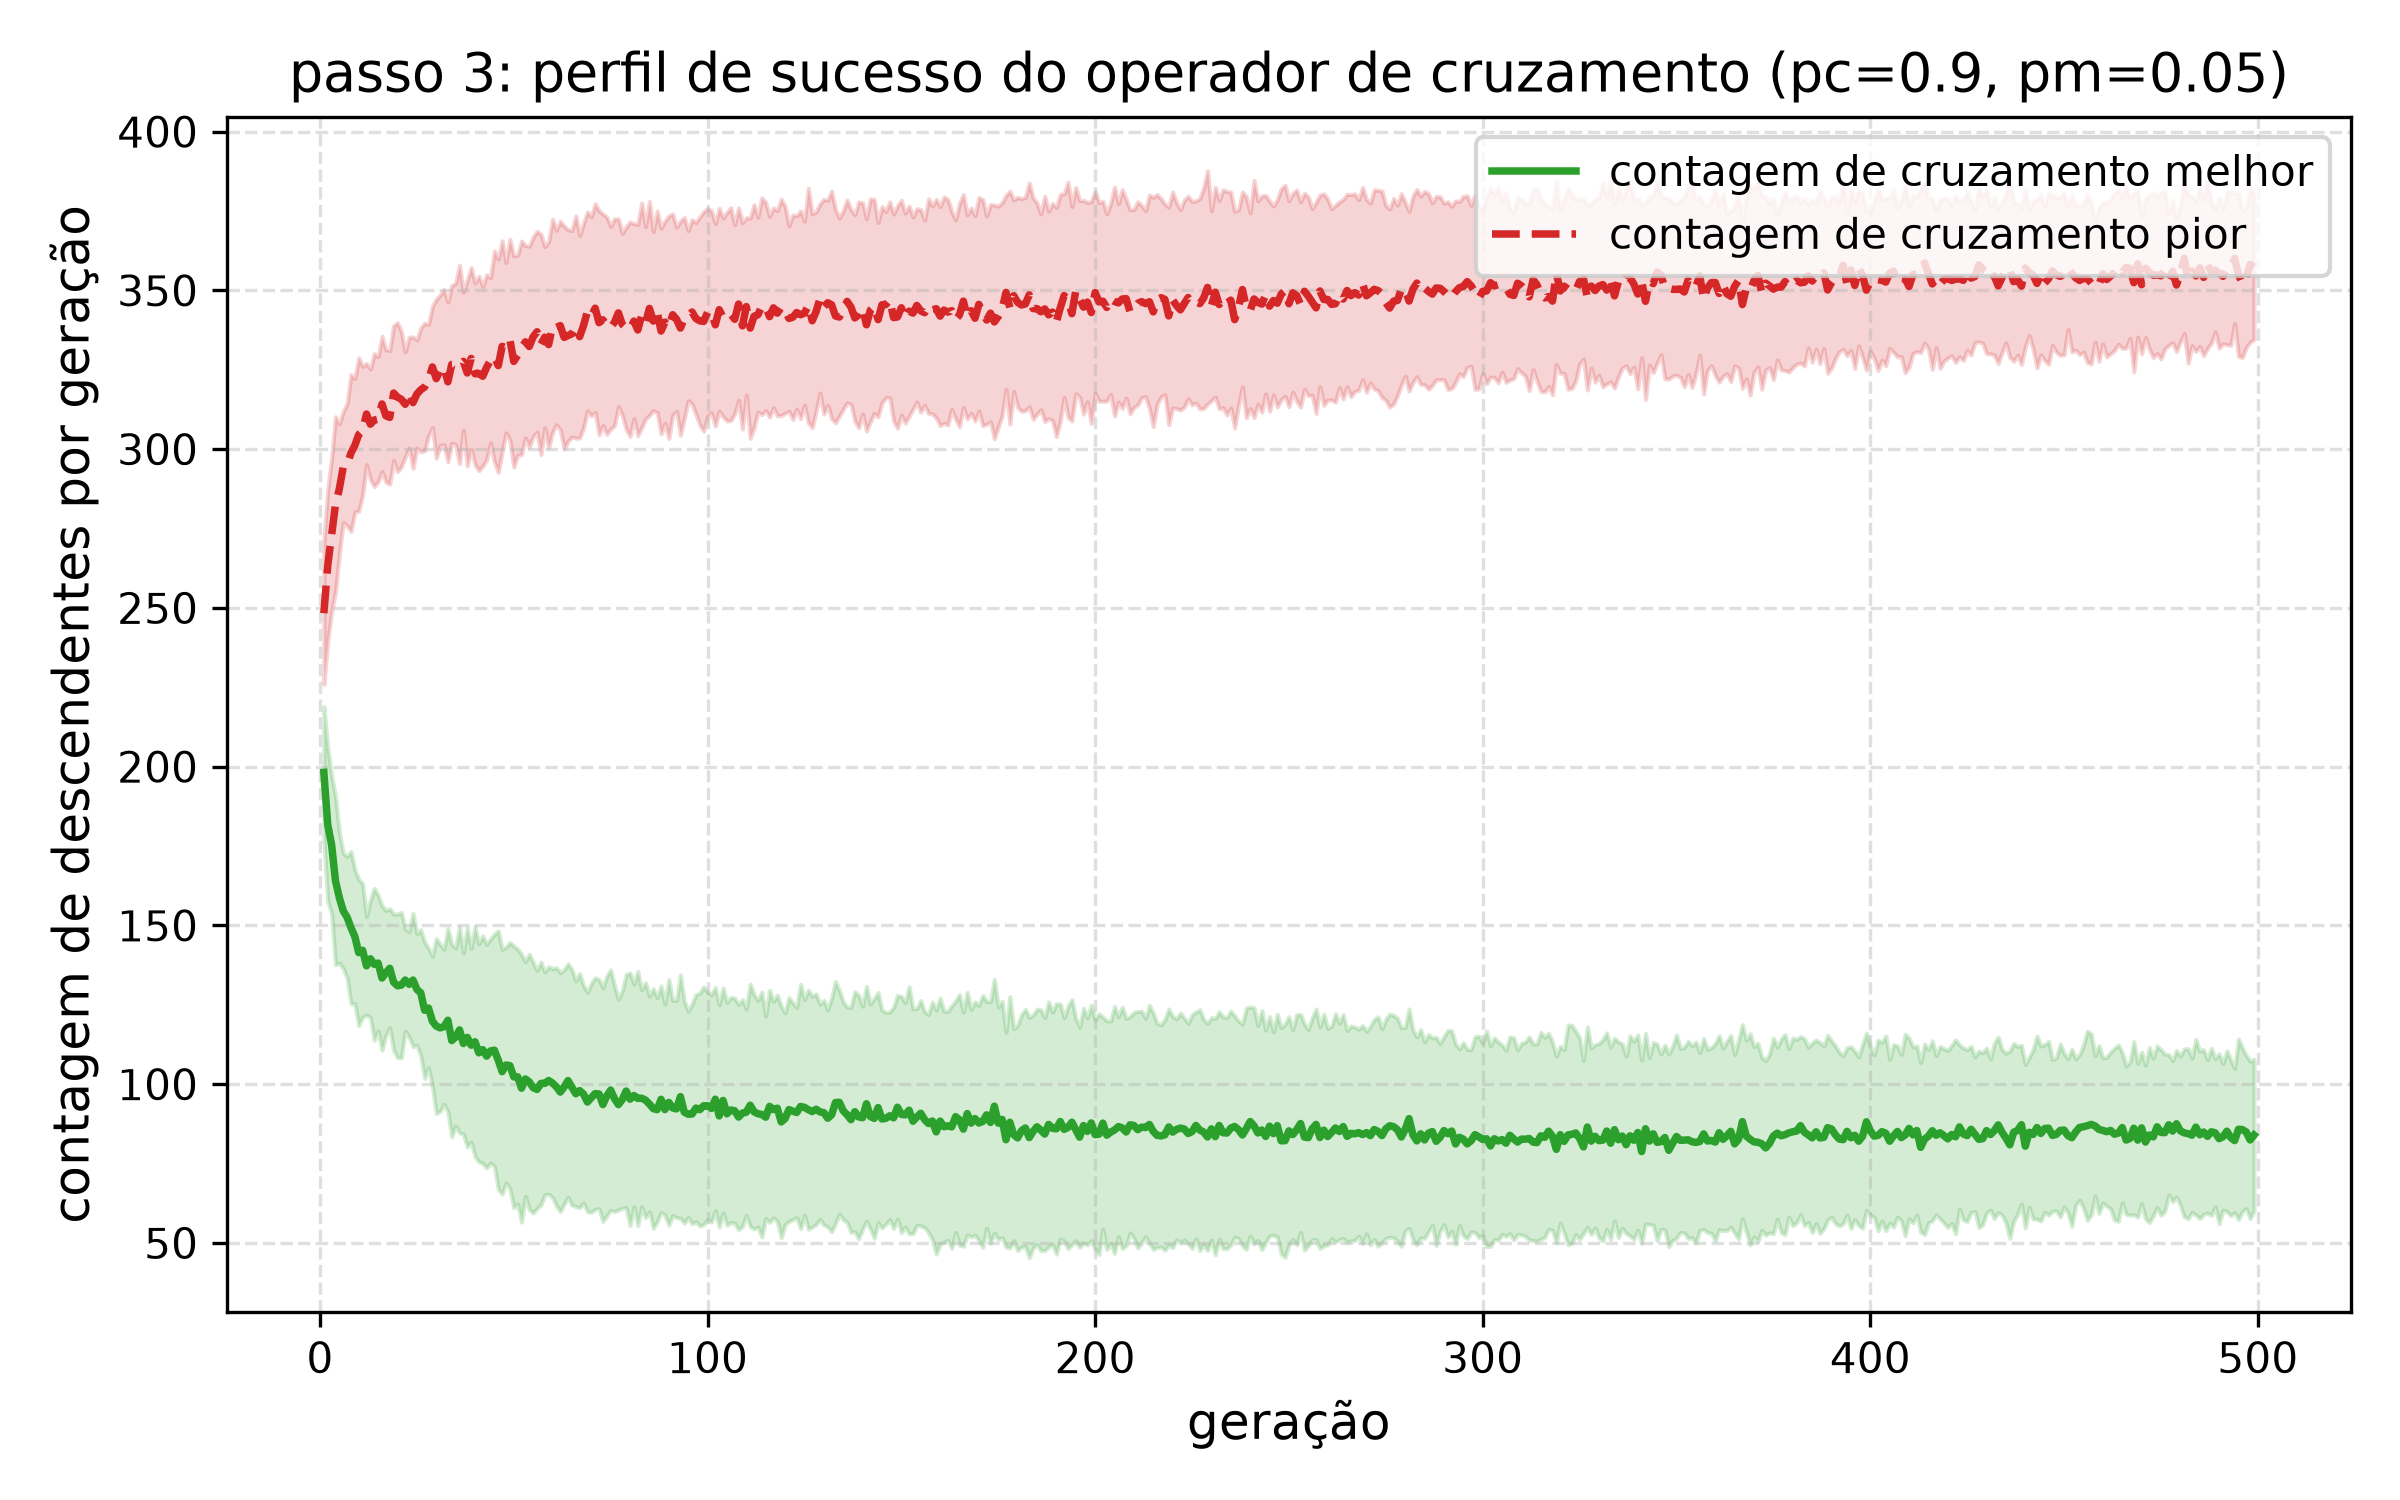
\includegraphics[width=0.85\textwidth]{results/plots/fig5_step3_operator_success.png}%
  }{%
    \fbox{\parbox{0.8\textwidth}{\centering Placeholder: Inserir \texttt{results/plots/fig5_step3_operator_success.png}}}%
  }
  \caption{Taxas de sucesso do crossover (filhos melhores vs. piores que os pais) ao longo das gerações.}
  \label{fig:step3_operators}
\end{figure}

\subsection{Análise do Impacto do Elitismo (Passo 4)}
% [ORIENTAÇÃO: Compare a trajetória de convergência com e sem elitismo.
% Destaque a perda temporária de soluções ótimas no regime sem elitismo e o efeito na estabilidade.]

% Inserção da Tabela 4:
% \begin{table}[htbp]
  \centering
  \caption{Resultados resumidos do Passo 4}
  \label{tab:step4}
  \begin{tabular}{llcccc}
    \toprule
    Configuration & Dataset & Train RMSE & Test RMSE & Avg Nodes & Avg Depth \\
    \midrule
    with\_elitism & synth1 & 0.2609 $\pm$ 0.3722 & 0.4927 $\pm$ 0.9241 & 36.27 $\pm$ 9.10 & 7.00 $\pm$ 0.00 \\
    without\_elitism & synth1 & 0.4902 $\pm$ 0.5729 & 0.9206 $\pm$ 1.2375 & 38.63 $\pm$ 9.68 & 6.97 $\pm$ 0.18 \\
    \bottomrule
  \end{tabular}
\end{table}


% Inserção da Figura 4 (Comparação de Elitismo):
\begin{figure}[htbp]
  \centering
  \IfFileExists{results/plots/fig6_step4_elitism_comparison.png}{%
    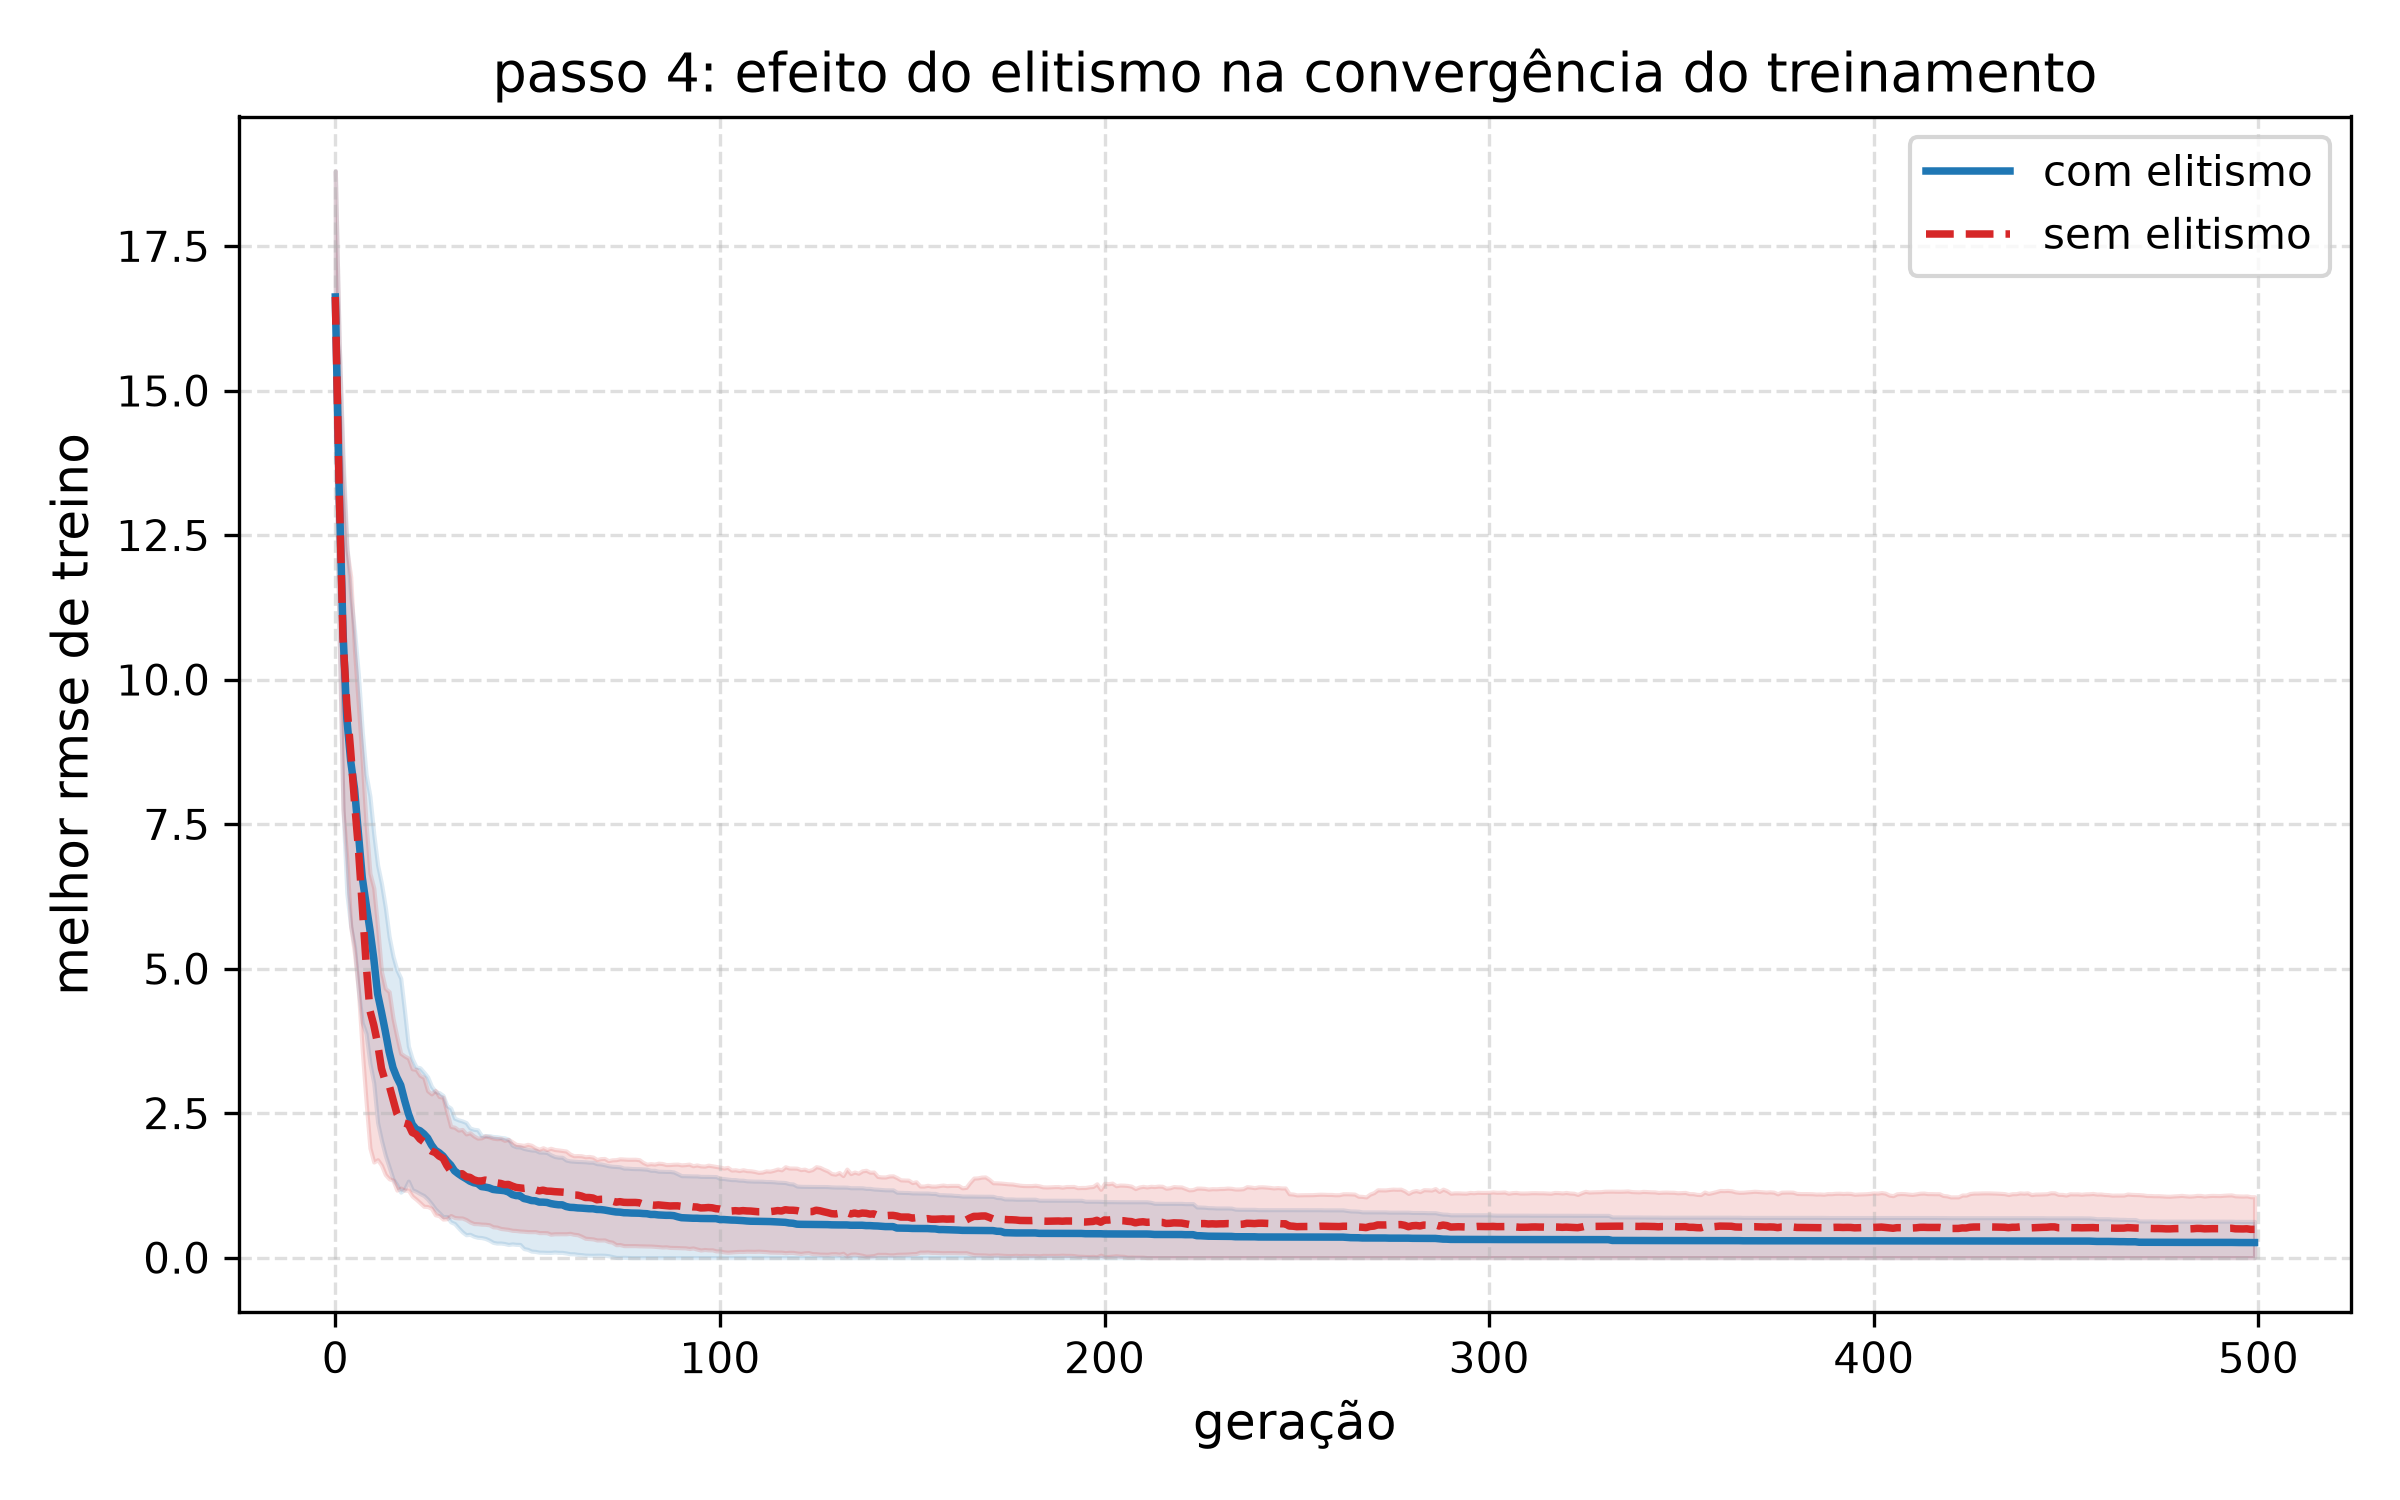
\includegraphics[width=0.85\textwidth]{results/plots/fig6_step4_elitism_comparison.png}%
  }{%
    \fbox{\parbox{0.8\textwidth}{\centering Placeholder: Inserir \texttt{results/plots/fig6_step4_elitism_comparison.png}}}%
  }
  \caption{Impacto do mecanismo de elitismo na estabilidade e monotonia da convergência do melhor indivíduo.}
  \label{fig:step4_elitism}
\end{figure}

\subsection{Validação Final nos Conjuntos synth2 e concrete (Passo 5)}
% [ORIENTAÇÃO: Apresente o desempenho da melhor configuração global sobre as bases synth2 e concrete.
% Compare o erro de treino e teste (gap de generalização) e analise a complexidade das expressões encontradas.]

% Inserção da Tabela 5:
% \begin{table}[htbp]
  \centering
  \caption{Resultados resumidos do Passo 5}
  \label{tab:step5}
  \begin{tabular}{llcccc}
    \toprule
    Configuration & Dataset & Train RMSE & Test RMSE & Avg Nodes & Avg Depth \\
    \midrule
    concrete & concrete & 7.9342 $\pm$ 0.3954 & 8.0103 $\pm$ 0.5213 & 42.50 $\pm$ 6.99 & 7.00 $\pm$ 0.00 \\
    synth2 & synth2 & 0.5726 $\pm$ 0.5876 & 0.6501 $\pm$ 0.6953 & 35.23 $\pm$ 7.81 & 6.93 $\pm$ 0.25 \\
    \bottomrule
  \end{tabular}
\end{table}


% Inserção da Figura 5 (Validação Final e Paridade):
\begin{figure}[htbp]
  \centering
  \IfFileExists{results/plots/fig7_step5_synth2_concrete_convergence.png}{%
    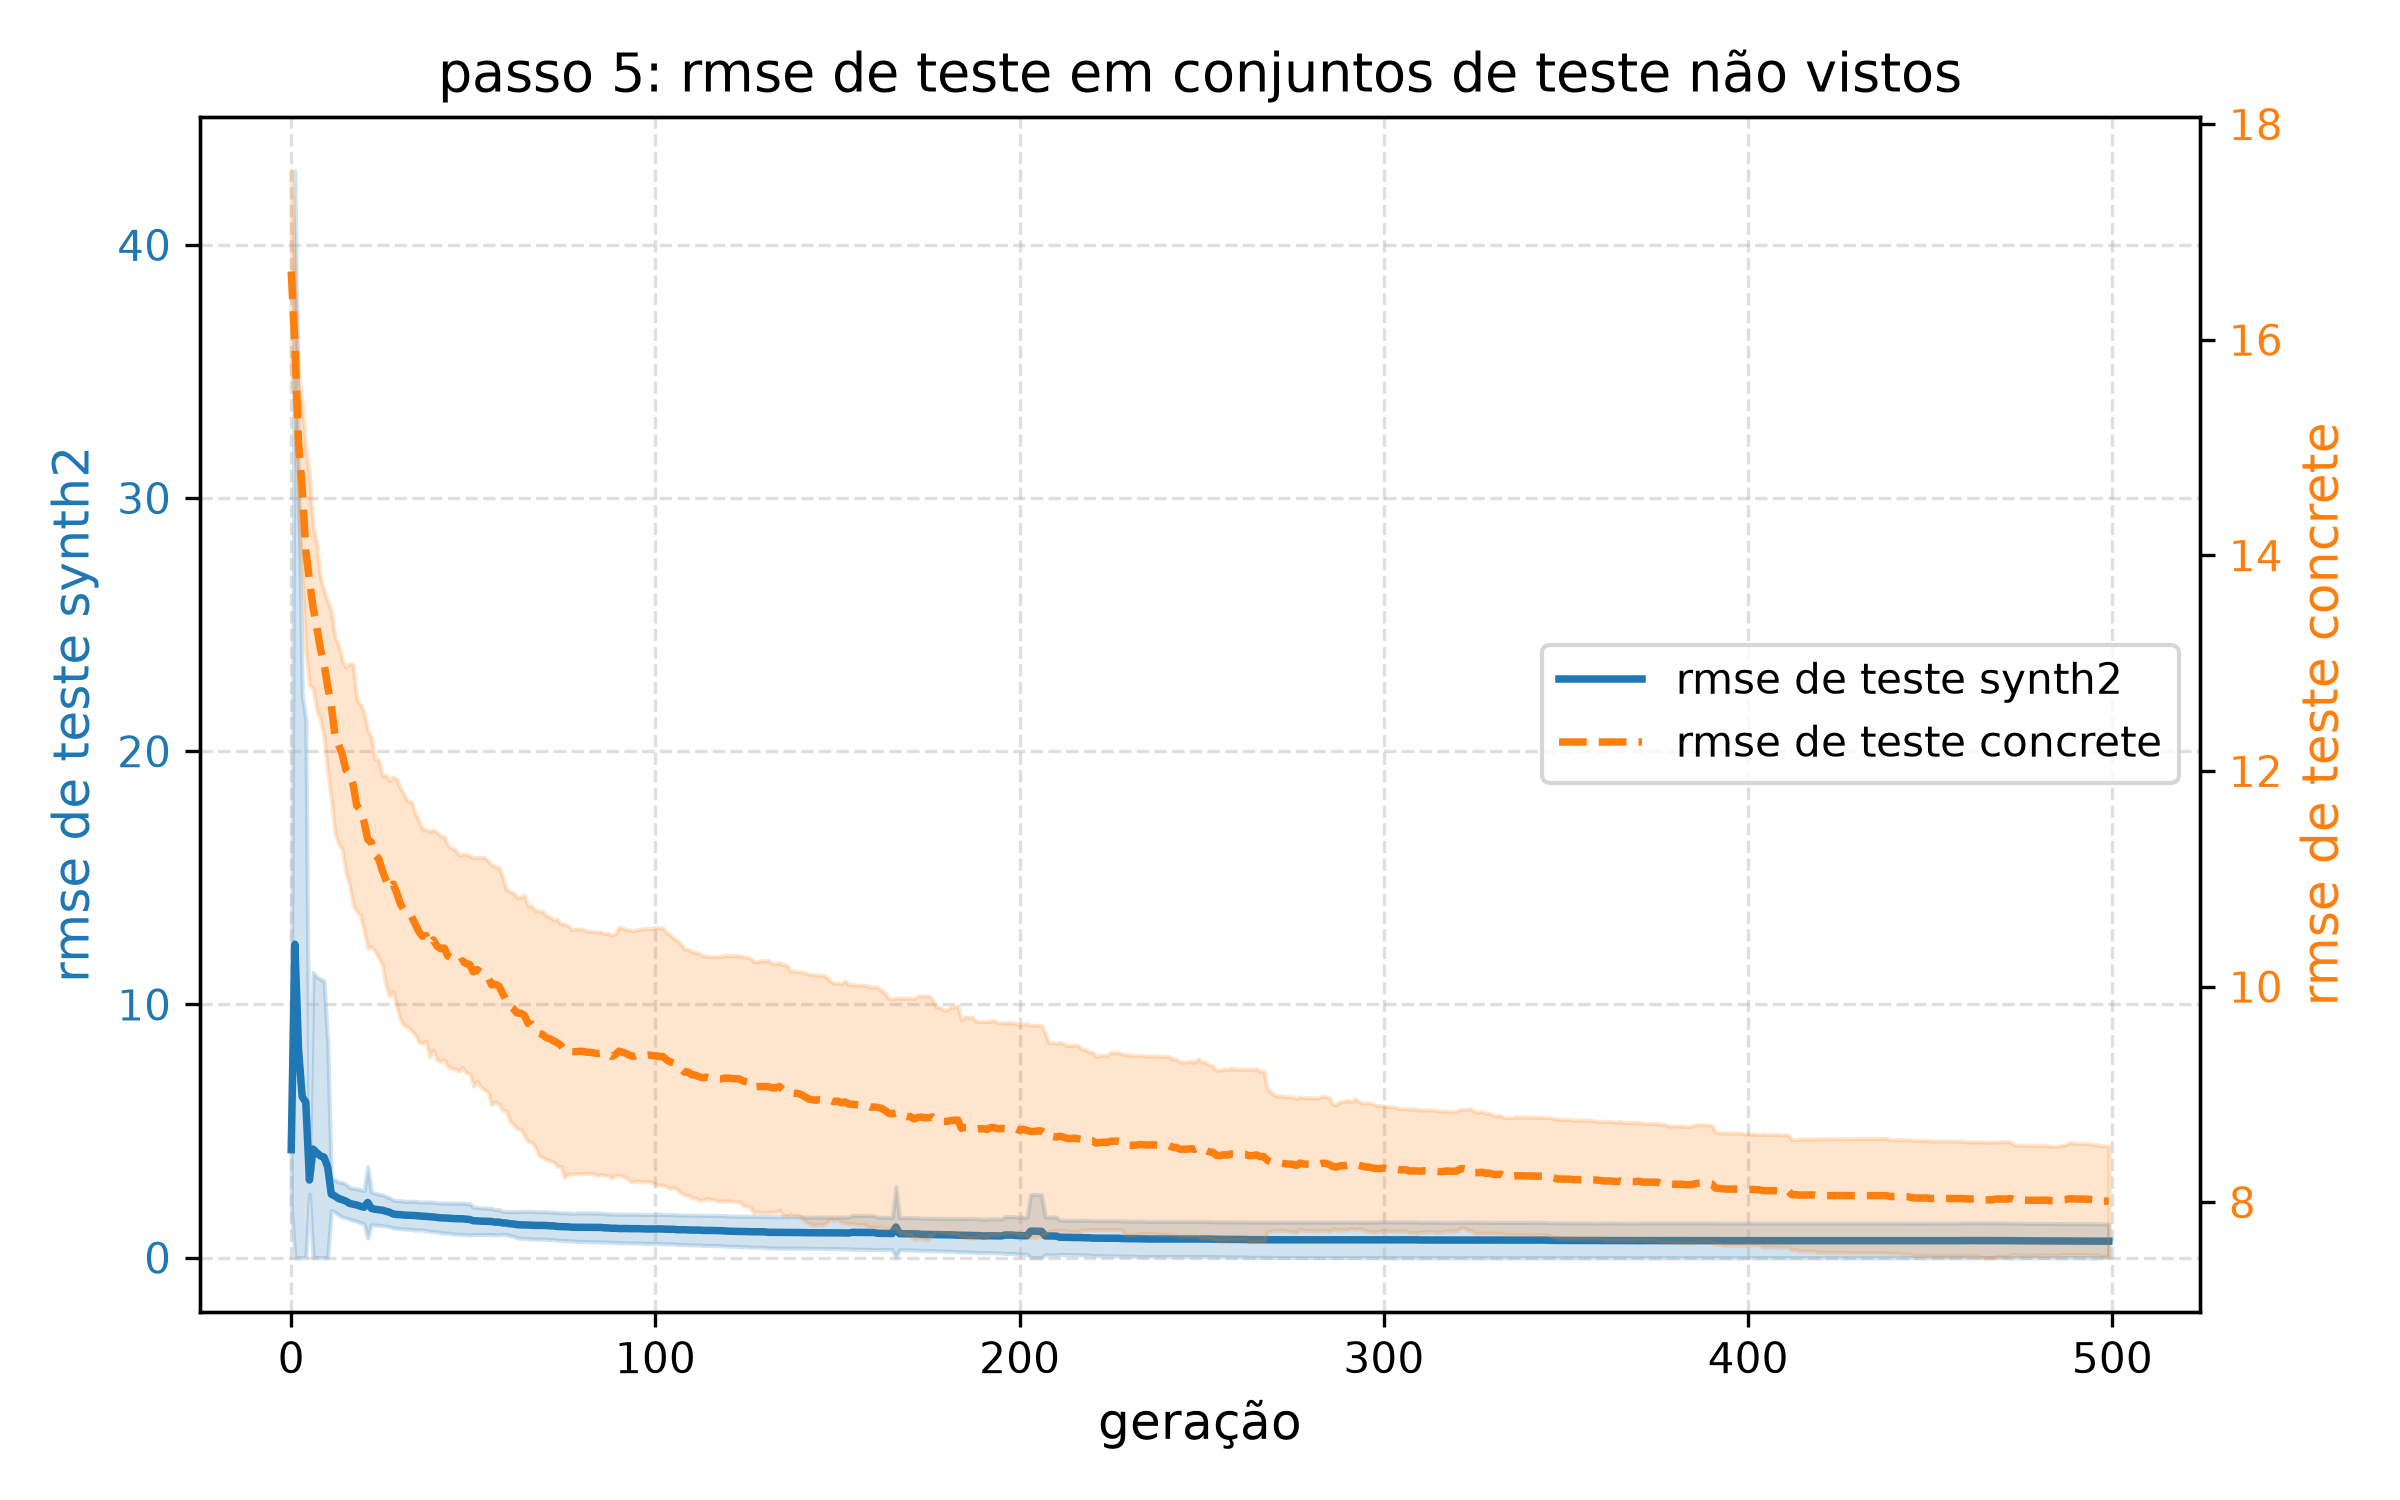
\includegraphics[width=0.85\textwidth]{results/plots/fig7_step5_synth2_concrete_convergence.png}%
  }{%
    \fbox{\parbox{0.8\textwidth}{\centering Placeholder: Inserir \texttt{results/plots/fig7_step5_synth2_concrete_convergence.png}}}%
  }
  \caption{Convergência final do RMSE de treino e teste nas bases synth2 e concrete.}
  \label{fig:step5_convergence}
\end{figure}

\begin{figure}[htbp]
  \centering
  \IfFileExists{results/plots/fig8_step5_generalization_scatter.png}{%
    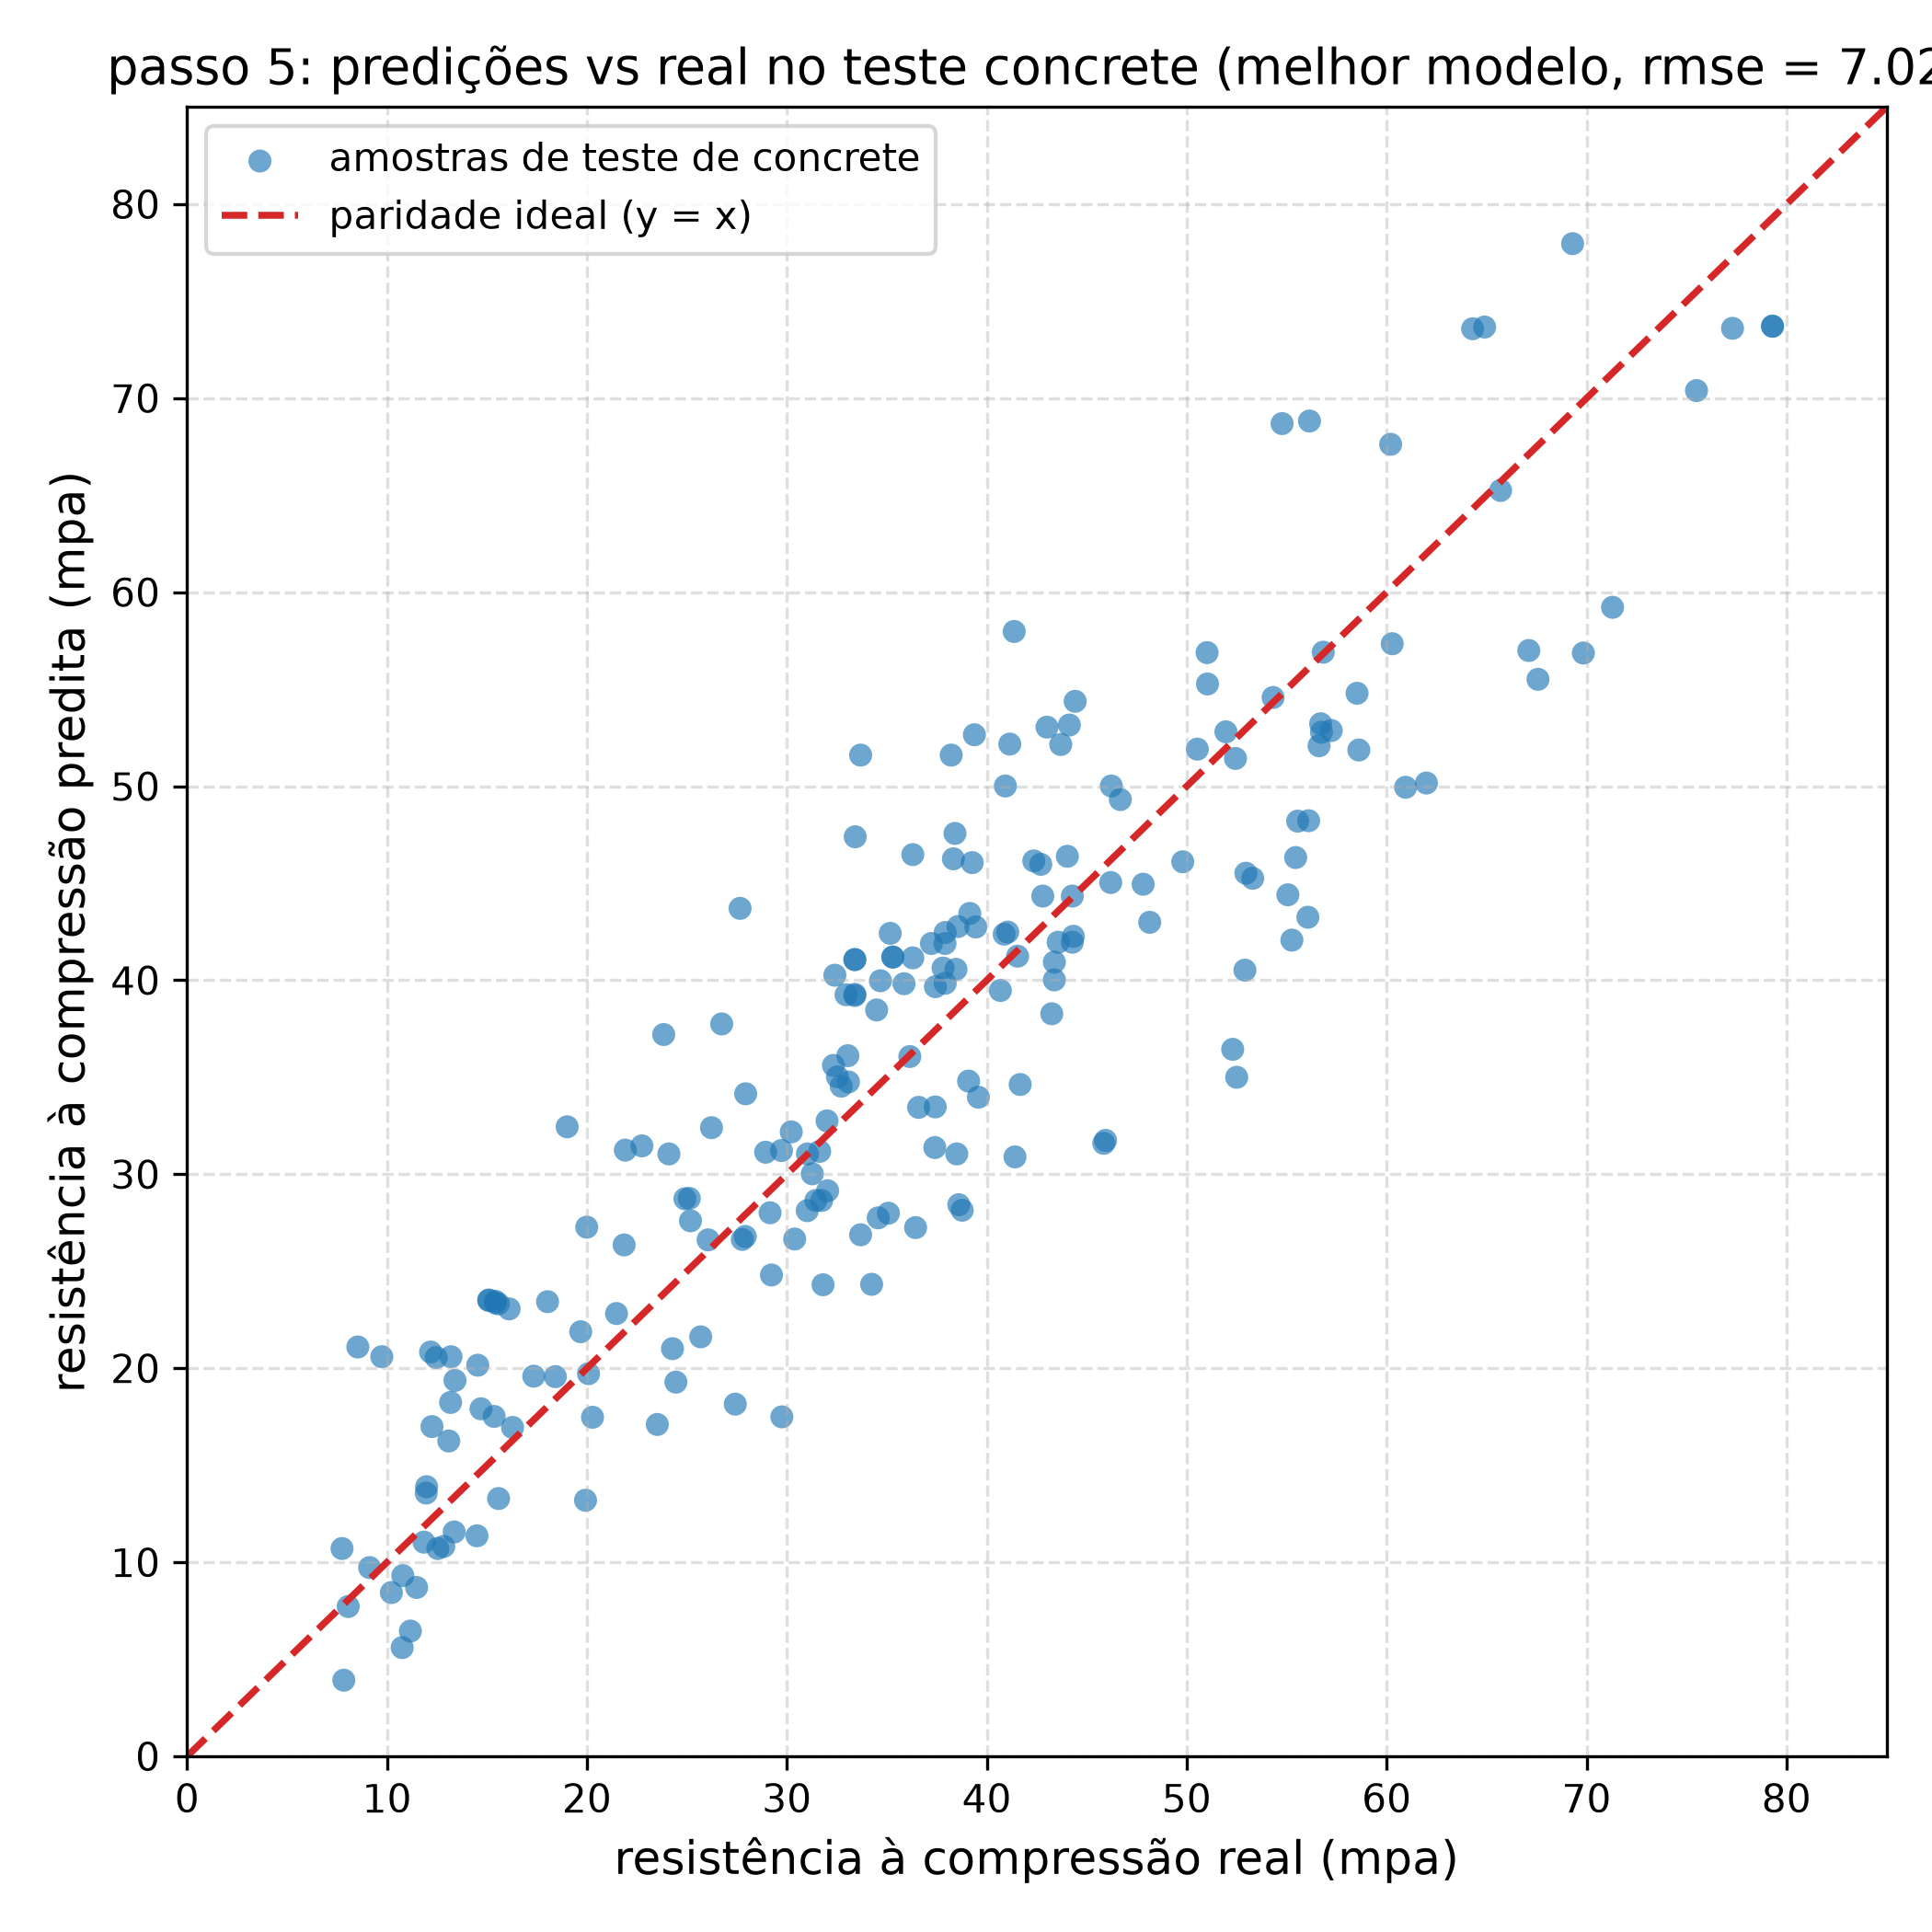
\includegraphics[width=0.85\textwidth]{results/plots/fig8_step5_generalization_scatter.png}%
  }{%
    \fbox{\parbox{0.8\textwidth}{\centering Placeholder: Inserir \texttt{results/plots/fig8_step5_generalization_scatter.png}}}%
  }
  \caption{Gráfico de paridade (valores previstos vs. valores reais) no conjunto de teste para o melhor modelo.}
  \label{fig:step5_parity}
\end{figure}

\section{Conclusões}
% [ORIENTAÇÃO: Sintetize as principais descobertas experimentais.
% Indique quais operadores e parâmetros se mostraram mais robustos para regressão simbólica.
% Discuta limitações encontradas (ex.: bloat, tempo de avaliação em bases maiores) e proponha melhorias futuras.]

\bibliographystyle{plain}
\bibliography{referencias}
\end{document}
